\documentclass[10pt]{article}
\usepackage[margin=0.85in]{geometry}
\usepackage{amsmath}
\usepackage{booktabs}
\usepackage{array}
\usepackage{graphicx}
\usepackage{float}
\usepackage{multicol}
\usepackage{xcolor}
\usepackage{tikz}
\usepackage{hyperref}
\hypersetup{colorlinks=true,linkcolor=blue!45!black,urlcolor=blue!45!black,
  pdftitle={Predicting Glanders Disease Across a Lifestyle or Geographical Area},
  pdfauthor={GlandersWatch Project Team},
  pdfsubject={Chained multi-level machine-learning evaluation}}
\usetikzlibrary{shapes.geometric,arrows.meta,positioning,fit,backgrounds,calc,decorations.pathreplacing}
\graphicspath{{../figures/}}
\setlength{\parskip}{0.28em}
\raggedbottom
\sloppy

\title{\textbf{Predicting Glanders Disease Across a Lifestyle or Geographical Area}\\[0.3em]
\large Chained Multi-Level Machine Learning on Four Unused Datasets}
\author{GlandersWatch Project Team}
\date{\today}

\begin{document}
\input{diagstyles.tex}
\maketitle

\noindent
\textbf{What this project does, in short.} Glanders is a dangerous bacterial disease of
horses and donkeys. We asked one question: can we predict, using only public data,
which countries will report glanders next year?

We combined four data sources that had never been used for this disease: published
research papers, farm animal counts, World Bank statistics, and NASA climate records.
We then trained six machine learning models and tested them on future years and on
countries the models had never seen.

The result is a working early-warning model. It ranks likely countries about ten times
better than random guessing, and its stated probabilities turned out to be trustworthy.
Warning only about 6\% of the world each year would catch roughly half of all reported
outbreaks. The honest limitations are that the model works less well in countries it has
not seen, and that it largely learns \emph{which countries report} disease rather than
\emph{where} disease is. Both points are discussed openly in Section~9.

% =====================================================================

% =====================================================================
\section{What We Tried To Do}
% =====================================================================

Glanders is a bacterial disease that kills horses, donkeys and mules, and it can pass to
people who handle infected animals. Most Indian equids belong to poor families who use
them for transport, farming and construction. A district officer who knew a year ahead
that glanders was likely could warn owners in time to act. So the question is:

\begin{quote}
\emph{Given what we know about a country this year, can we predict whether glanders
will be reported there next year?}
\end{quote}

One row in our data is one country in one year. The model returns a number between 0 and
1, which we read as a risk score. A score of 0.30 means roughly a 30\% chance that
glanders will be reported in that country next year.

The model does not diagnose an animal and cannot tell a farmer whether their horse is
sick. It works at the level of countries and years, so it suits planning work. It is not
a substitute for a veterinarian looking at a sick animal.

% =====================================================================

\section{Related Work}
\label{sec:related}

\textbf{Glanders.} A neglected zoonosis of equids with high mortality and real human risk
\cite{khan2013,kanani2026}; a 2026 meta-analysis consolidates seroprevalence and names
management and movement as the main drivers \cite{purnama2026}. Brazil keeps an active
control literature \cite{mota2022}.

\textbf{India.} Outbreaks 2006--11 \cite{malik2012}, serosurveillance 2015--18
\cite{singha2020}, and a multi-state survey 2019--23 \cite{singha2026} establish
\emph{where} glanders is. None builds a predictive model.

\textbf{Geographic risk.} Spatiotemporal cluster detection for Brazilian glanders
\cite{fonseca2019} and niche models for livestock disease \cite{hollings2017} are both
descriptive: clusters are found after the fact, not forecast.

\textbf{ML for animal disease.} The closest template is avian influenza: ARIMA versus
random forest \cite{kane2014}, ML-targeted surveillance \cite{walsh2019}, dynamic farm-level
risk \cite{yoo2022}, and an outbreak model for Kuwait \cite{alshatti2026}. That template
exists for influenza, not glanders.

\textbf{The gap.} The only ML on \emph{B.\ mallei} is spectroscopic identification of the
organism \cite{moawad2019,stoeckel2015}, which is a laboratory test rather than a population
forecast.
Text mining has precedent in epidemic intelligence \cite{collier2012,lejeune2015}, but not
for glanders.

\textbf{Methods.} Random forests \cite{breiman2001}, XGBoost \cite{chen2016} and LightGBM
\cite{ke2017}, explained with SHAP \cite{lundberg2017}. Rare events call for
precision-recall \cite{saito2015,davis2006}; probabilities are calibrated
\cite{niculescu2005,huang2020}; validation respects temporal and spatial dependence
\cite{roberts2017}. Data: WAHIS \cite{wahis}, India's 2025 action plan \cite{dahd2025},
FAOSTAT \cite{faostat}, World Bank \cite{wdi}, NASA POWER \cite{power}, Europe PMC
\cite{europepmc}.

\textbf{Position.} Prior glanders work is descriptive or laboratory-based, prior veterinary
ML is built for influenza, and text-mined occurrence has never been used for glanders. This
study joins all four and reports what predicts and what does not.

\section{Dataset Used}
% =====================================================================

We used four public data sources. None had been used for glanders before, which is the
main reason this counts as new work.

\begin{table}[htbp]
\centering
\caption{The four data sources. Glanders events in Europe PMC were extracted by
matching a country name and an event term within the same sentence, which yielded 263
events across 2000 to 2024.}
\small
\begin{tabular}{@{}>{\raggedright\arraybackslash}p{5.6cm}>{\raggedright\arraybackslash}p{3.6cm}>{\raggedright\arraybackslash}p{4.8cm}@{}}
\toprule
\textbf{Source} & \textbf{What it gives us} & \textbf{Size} \\
\midrule
Europe PMC (research papers) & Where and when glanders was reported & 6,674 papers $\rightarrow$ 263 events \\
FAOSTAT & How many horses, donkeys, mules, cattle, goats and sheep each country has & 68,449 records, 1961--2023 \\
World Bank & Money, farming, population, internet access & 10 indicators, 217 countries \\
NASA POWER & Temperature, rainfall, humidity, wind & 6 measures, 211 locations \\
\bottomrule
\end{tabular}
\end{table}

\paragraph{Why these four sources.} They cover what decides whether a disease can appear at
all: whether it has been there before, how many animals could catch it, and whether the
climate suits it. World Bank data adds a rough measure of how well a country detects and
reports disease. Pulling several kinds of data together is what makes this stronger than an
analysis of one source.

\paragraph{The assembled panel.} All four sources are keyed on ISO-3 country code and
calendar year, so they join without ambiguity. The full panel has 6,700 country-year
rows covering 268 countries from 2000 to 2024. For modelling we keep only
equine-holding countries, meaning those with a maximum stock of at least 1{,}000 equids, the
years 2005 to 2023, and rows where next year's answer is observable. That leaves
\textbf{3,078 rows, 44 input columns and 172 positive labels}.

\paragraph{Preprocessing.} Five steps, in this order.

\begin{enumerate}
\setlength{\itemsep}{0.1em}
\item \textbf{Name reconciliation.} Country and area names were matched across sources
      through \texttt{pycountry} with explicit overrides, because the same country is
      written ``T\"urkiye'' in one file and ``Turkey'' in another. Without this the joins
      would silently drop rows.
\item \textbf{Aggregate removal.} World Bank regional and global totals were dropped by
      requiring a three-character ISO code, so rows such as ``World'' and ``South Asia''
      cannot enter the panel as if they were countries.
\item \textbf{De-duplication.} Literature events were de-duplicated on the key
      \texttt{(iso3, year, record\_id)}, so one paper cannot inflate a cell by being
      counted several times.
\item \textbf{Missing values.} Filled with the column median, and every column keeps a
      missing-indicator flag so the model can tell an imputed value from a real one. The
      fill is fitted inside the training pipeline, never on the full table. Missing data
      was rare: 0.99\% overall and 5.8\% in the worst column.
\item \textbf{Absence handling.} A country-year is coded 0 only after that country passes
      the equine-stock filter, so a blank is never read as proof that disease was absent.
      This is the step that keeps the label honest.
\end{enumerate}

\paragraph{Feature engineering.} Four groups of columns were built from the raw sources,
all using information available in the current year or earlier. History columns are lags, a
five-year running total and years since the last event. Population columns add derived
quantities: equid share of all farm animals, equine density, and growth over one and three
years. Climate columns pair each measure with an anomaly, its deviation from that country's
own expanding mean. Section~\ref{sec:features} lists all four groups.

\paragraph{Feature selection.} Every input was screened for association with the answer and
for duplication of another input, but the screens were read rather than obeyed. Only one column
was dropped outright: total equids, because it is exactly the sum of horses, asses and mules and a
tree can rebuild it. Four columns scored below both association thresholds and three near-duplicate
pairs were flagged, yet all were kept, for the reason covered in Section~\ref{sec:analysis}: the
univariate screen disagrees with what the fitted model actually uses, and one flagged column turns
out to be among the three most important. No principal component analysis was used either; the
limit here is signal rather than dimensionality.

% =====================================================================
\section{Dataset Analysis}
\label{sec:analysis}
% =====================================================================

We start with the label, then move to how each input relates to it and how much the inputs
duplicate each other.

\paragraph{The answer key.} For every country and year the answer is yes or no: was
glanders reported the following year? Only 172 of the 3,078 rows are yes, which is 5.6\%.

\begin{table}[htbp]
\centering
\caption{Numbers describing the answer key.}
\small
\begin{tabular}{@{}lr@{}}
\toprule
\textbf{Measure} & \textbf{Value} \\
\midrule
Total rows & 3,078 \\
``Yes'' rows (event next year) & 172 \\
``No'' rows & 2,906 \\
Percentage ``yes'' & 5.6\% \\
Ratio of no to yes & about 17 to 1 \\
Countries with at least one ``yes'' & 56 of 162 \\
Countries with ``yes'' in two or more years & 30 \\
Share of all ``yes'' in the top 5 countries & 35.5\% \\
\bottomrule
\end{tabular}
\end{table}

\paragraph{What the distribution tells us.} Three things follow from that table, and each
one changed a decision later. First, yes is rare enough that always answering no would be
right 94.4\% of the time, so accuracy is useless here and we need scores built for rare
events. Second, the disease comes back: 30 of the 56 positive countries were positive in
two or more years, so past activity is a fair input rather than a shortcut. Third, the yes
answers cluster, with five countries holding 35.5\% of them, and those five are mostly rich
countries that run publishing laboratories.

For that reason the target is termed \emph{documented activity} rather than
\emph{disease occurrence}. A negative label can reflect either the absence of disease or the
absence of a report.

Before training anything we measured how each input relates to the answer. Three measures
were used on the numeric columns.
\emph{Spearman's $\rho$} checks whether two quantities rise and fall together, on a scale
from $-1$ to $+1$. \emph{Mutual information} catches relationships that are not a straight
line, and equals zero when a column tells you nothing about the answer. \emph{Cram\'er's
$V$} does the same job for text categories such as region.

\paragraph{Statistical association.} The strongest monotone signal in the whole dataset is
\texttt{years\_since\_last} at $\rho = -0.35$. The sign is negative because more years
since the last outbreak means lower risk. This is the one broadly epidemiological result in
the panel, and it says what we would hope: recent activity predicts future activity. On the
same scale, \texttt{internet\_pct} scores only $+0.09$ and \texttt{temp\_mean\_anom} about
zero. For the two text categories, region gives Cram\'er's $V$ of 0.243, which counts
as a small association, and income band gives 0.047, which is negligible. Neither is
strong enough to act as a stand-in for the label.

\paragraph{Correlation and redundancy.} Several columns measure nearly the same thing.
Variance inflation factor is the standard measure of that, where a value above 10 is
usually treated as a problem. It reaches 228 for \texttt{temp\_mean}, because annual mean,
minimum and maximum temperature are near-duplicates of each other at country resolution.
Three groups sit at $|\rho| \geq 0.90$: \texttt{occ\_lag1} with \texttt{occ\_count\_lag1},
\texttt{cattle} with \texttt{log\_livestock}, and \texttt{temp\_mean} with \texttt{temp\_min}.
We kept one member of each group. This matters for reading coefficients in a linear model,
and not much for trees, since a tree splits on thresholds and does not care whether two
columns carry overlapping information.

\paragraph{Where the two importance measures disagree.} This is the result that shaped the
whole feature set. We compared how much each column correlates with the answer on its own
with how much the trained model actually relies on it, using SHAP. The two rankings agreed
almost not at all, with a rank correlation of +0.31 and only 5 of the 10 top features
shared. Longitude is the clearest case: it ranks first on simple correlation and around
twentieth in what the model uses. The explanation is that longitude does not cause
glanders. It identifies which part of the world a country is in, and some parts publish
more papers. Ranking features by marginal correlation would therefore favour columns that
track reporting practice rather than disease occurrence. Features were selected on the
conditional evidence instead, and correlation was used only to discard columns with no
signal.

\begin{table}[htbp]
\centering
\caption{Top 8 features by importance to the trained model, with marginal statistics
alongside. The gap between the two sets of numbers is the disagreement described above.}
\small
\resizebox{\textwidth}{!}{%
\begin{tabular}{@{}rlrrrr@{}}
\toprule
\textbf{Rank} & \textbf{Feature} & \textbf{Importance} & \textbf{Correlation} & \textbf{Mutual info} & \textbf{Redundancy} \\
 & & \textbf{(mean $|$SHAP$|$)} & \textbf{(Spearman $\rho$)} & \textbf{(MI)} & \textbf{(VIF)} \\
\midrule
1 & pop\_total & 1.476 & +0.28 & 0.0639 & 4 \\
2 & internet\_pct & 0.896 & +0.09 & 0.0015 & 5 \\
3 & goats & 0.661 & +0.19 & 0.0422 & 27 \\
4 & log\_livestock & 0.626 & +0.25 & 0.0571 & 3 \\
5 & precip\_cv & 0.609 & -0.01 & 0.0006 & 2 \\
6 & temp\_mean\_anom & 0.598 & -0.00 & 0.0012 & 2 \\
7 & years\_since\_last & 0.576 & -0.35 & 0.0486 & 2 \\
8 & cattle & 0.548 & +0.25 & 0.0512 & 7 \\
\bottomrule
\end{tabular}}
\end{table}

\paragraph{What we removed, and why.} Four columns had mutual information below 0.002 and
$|\rho|$ below 0.02, which means no measurable relationship to the answer at all. We
dropped one column that was exactly the sum of three others, since it adds nothing a tree
cannot build itself. We dropped one member of each near-duplicate pair listed above. No
principal component analysis was used: with 44 columns and 3,078 rows the limit is signal
rather than dimensionality, and the section on results confirms that fewer columns
generalise better across countries, so compressing further would have cost
interpretability for nothing. Scaling is applied only to the logistic baseline, because
tree models are indifferent to it.

% =====================================================================
\section{What We Gave The Model (Features)}
\label{sec:features}
% =====================================================================

A feature is an input column. Forty-four were engineered and fourteen are used, all of them built
from information available in the current year or earlier. The candidates fall into four groups.

\begin{itemize}
\setlength{\itemsep}{0.15em}
\item \textbf{Disease history (7 columns).} Outbreaks in the previous two years, the
      five-year running total, years since the last event, and world and regional activity
      shares for the same year. The disease persists once introduced, so this group carries
      the epidemiological prior.
\item \textbf{Animal population (14 columns).} Log equid and total livestock stocks, the
      equid share of all farm animals, equid density, growth over one and three years, and
      the seven species counts. More animals means more chances to find the disease.
\item \textbf{Climate (10 columns).} Mean, maximum and minimum temperature, precipitation
      total and its coefficient of variation, relative humidity, and wind, each paired with
      an \emph{anomaly}. An anomaly is the difference from that country's own expanding
      mean, which separates ``unusually wet for here'' from an absolute number that mostly
      encodes latitude.
\item \textbf{Country context (11 columns).} Income band, agricultural land share,
      agricultural value added, livestock production index, GDP per person, rural share,
      internet penetration, fertiliser intensity, life expectancy, population and density.
      These mostly measure how well a country detects disease.
\end{itemize}

Three derived columns are worth naming. \emph{Equid share} is horses plus donkeys plus
mules divided by all farm animals, which shows how much of the farming depends on equids.
\emph{Livestock units} counts cattle and camels at full weight and small ruminants at one
tenth, following standard metabolic weights, so one number expresses grazing pressure
across species. \emph{Years since last event} uses 99 to mean ``never recorded''.

% =====================================================================
\section{Models We Tried}
% =====================================================================

We trained six models, including a deliberately simple one to compare against. The table
gives each model's family, what it does, and the settings the tuning search picked.

\begin{table}[htbp]
\centering
\caption{The six models, their family, and the settings chosen by tuning.}
\small
\begin{tabular}{@{}>{\raggedright\arraybackslash}p{2.9cm}>{\raggedright\arraybackslash}p{2.3cm}>{\raggedright\arraybackslash}p{8.9cm}@{}}
\toprule
\textbf{Model} & \textbf{Family} & \textbf{What it does, and the settings chosen} \\
\midrule
Logistic Regression & linear & Adds the inputs with fixed weights and squashes the total into a 0--1 score. The honest baseline: if the complex models cannot beat it, the complexity is not worth it.\par\vspace{3pt}{\scriptsize Tuned settings: \emph{$C=1.0$, $\ell_2$ penalty, balanced class weights}} \\
Decision Tree & tree & A flowchart of yes/no questions, for example ``horses $>$ 10,000? then last outbreak $<$ 2 years ago?''. Easy to read, but one tree is weak, which is part of why we included it.\par\vspace{3pt}{\scriptsize Tuned settings: \emph{depth 4, minimum leaf size 40, split criterion entropy}} \\
Random Forest & bagged trees & 500 trees, each trained on a random part of the data, then they vote. Fixes the single tree's habit of memorising.\par\vspace{3pt}{\scriptsize Tuned settings: \emph{depth 6, minimum leaf size 10, features per split 0.3}} \\
Extra Trees & bagged trees & Same idea, with splits chosen more randomly. Extra randomness helps when examples are scarce, as they are here.\par\vspace{3pt}{\scriptsize Tuned settings: \emph{depth 6, minimum leaf size 10, features per split 0.3}} \\
XGBoost & boosted trees & Trees built one after another, each fixing the previous mistakes. The strongest standard method for tables like ours.\par\vspace{3pt}{\scriptsize Tuned settings: \emph{depth 3, regularisation $\lambda=1.0$, minimum child weight 5}} \\
LightGBM & boosted trees & Same family as XGBoost with a faster algorithm. A speed comparison, often slightly better on wide data.\par\vspace{3pt}{\scriptsize Tuned settings: \emph{leaves 31, minimum child samples 40, regularisation $\lambda=3.0$}} \\
\bottomrule
\end{tabular}
\end{table}

Forest models train many trees \emph{in parallel} on random subsets and average them,
which reduces variance. Boosted models train trees \emph{in sequence}, each fitting the
error left by the last, which reduces bias. That difference explains why the two families
end up with similar scores.

We left neural networks out because the data cannot support them. With 172 positives and
44 inputs, a network has far more settings to learn than it has examples to learn from,
so it would memorise the training rows and fail on new ones. That is an argument from the
data rather than a judgement about the method.

The collinear columns noted in Section~\ref{sec:analysis} needed no special handling, since
trees split on thresholds.

\paragraph{How the final model was chosen.} On performance in countries it had never seen,
because that is how the model would be used. Extra Trees came out best at 0.363. Random
Forest scored higher on the easier time-based test, but the country test is the one that
speaks to deployment.

We did not stack the models into a meta-learner. The gap between families is smaller than
the uncertainty on any single score, so a meta-learner trained on 172 positives would add
variance without a gain we could defend. We spent that effort on calibration instead, since
that is what a threshold-based alert depends on.

% =====================================================================
\section{How We Trained And Tested It}
\label{sec:eval}
% =====================================================================

Several measures were taken so that nothing from the test period could influence training.

We ran three tests, and each answers a different question. They disagree for an
informative reason: the country split always scores lower than the time split, and that
gap is the price of meeting a country the model has never seen.


\begin{figure}[htbp]
\centering
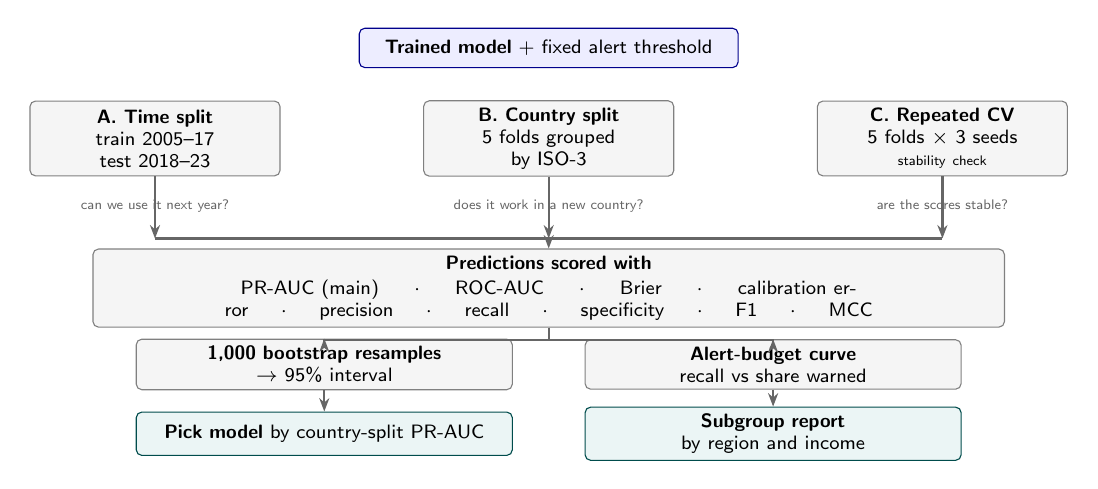
\begin{tikzpicture}[
  bx/.style={rectangle,rounded corners=2pt,draw=black!50,fill=black!4,
             align=center,font=\scriptsize\sffamily,inner sep=2.5pt},
  top/.style={rectangle,rounded corners=2pt,draw=blue!55!black,fill=blue!7,
             align=center,font=\scriptsize\sffamily,inner sep=3pt},
  fin/.style={rectangle,rounded corners=2pt,draw=teal!60!black,fill=teal!8,
             align=center,font=\scriptsize\sffamily,inner sep=2.5pt},
  fl/.style={-{Stealth[length=1.7mm]},thick,draw=black!60},
]

  \node[top,text width=4.6cm,minimum height=0.5cm] (m) at (0,0)
       {\textbf{Trained model} + fixed alert threshold};

  % three schemes
  \node[bx,text width=3.0cm,minimum height=0.95cm] (s1) at (-5.0,-1.15)
       {\textbf{A. Time split}\\train 2005--17\\test 2018--23};
  \node[bx,text width=3.0cm,minimum height=0.95cm] (s2) at (0,-1.15)
       {\textbf{B. Country split}\\5 folds grouped\\by ISO-3};
  \node[bx,text width=3.0cm,minimum height=0.95cm] (s3) at (5.0,-1.15)
       {\textbf{C. Repeated CV}\\5 folds $\times$ 3 seeds\\\tiny stability check};

  \node[font=\tiny\sffamily,text=black!60,anchor=north,text width=3.0cm,align=center] (q1)
       at (-5.0,-1.80) {can we use it next year?};
  \node[font=\tiny\sffamily,text=black!60,anchor=north,text width=3.0cm,align=center] (q2)
       at (0,-1.80) {does it work in a new country?};
  \node[font=\tiny\sffamily,text=black!60,anchor=north,text width=3.0cm,align=center] (q3)
       at (5.0,-1.80) {are the scores stable?};

  % collector rail
  \coordinate (railL) at (-5.0,-2.42);
  \coordinate (railR) at (5.0,-2.42);
  \draw[fl] (s1.south) -- (railL);
  \draw[fl] (s2.south) -- (0,-2.42);
  \draw[fl] (s3.south) -- (railR);
  \draw[thick,draw=black!60] (railL) -- (railR);

  \node[bx,text width=11.4cm,minimum height=0.78cm] (met) at (0,-3.05)
       {\textbf{Predictions scored with}\\[1pt]
        PR-AUC (main) $\;\cdot\;$ ROC-AUC $\;\cdot\;$ Brier $\;\cdot\;$ calibration error
        $\;\cdot\;$ precision $\;\cdot\;$ recall $\;\cdot\;$ specificity $\;\cdot\;$ F1
        $\;\cdot\;$ MCC};
  \draw[fl] (0,-2.42) -- (met.north);

  \node[bx,text width=4.6cm,minimum height=0.62cm] (boot) at (-2.85,-4.02)
       {\textbf{1{,}000 bootstrap resamples}\\$\rightarrow$ 95\% interval};
  \node[bx,text width=4.6cm,minimum height=0.62cm] (alert) at (2.85,-4.02)
       {\textbf{Alert-budget curve}\\recall vs share warned};

  \node[fin,text width=4.6cm,minimum height=0.55cm] (pick) at (-2.85,-4.90)
       {\textbf{Pick model} by country-split PR-AUC};
  \node[fin,text width=4.6cm,minimum height=0.55cm] (sub) at (2.85,-4.90)
       {\textbf{Subgroup report}\\by region and income};

  \draw[fl] (met.south) -- ++(0,-0.16) -| (boot.north);
  \draw[fl] (met.south) -- ++(0,-0.16) -| (alert.north);
  \draw[fl] (boot) -- (pick);
  \draw[fl] (alert) -- (sub);

\end{tikzpicture}
\caption{Evaluation pipeline. One trained model is scored three different ways, each
answering a different question, then reported with uncertainty intervals.}
\label{fig:evalflow}
\end{figure}


A random split would put the same country in both training and testing, which lets the
model memorise country patterns and look good for the wrong reason. Grouping by country
prevents that. The scores are defined in the glossary. In short, PR-AUC is the main one
because rare yes rows are what we care about, ROC-AUC is reported so others can compare,
and Brier plus calibration error check whether the percentages are believable.

Five things stayed inside the training data: model settings, the alert threshold, the
calibration step, the missing-value fill, and the choice of which columns to drop. The test
years could not touch any of them. Every input comes from the current year or earlier, with
only the answer taken from the following year.


\begin{figure}[htbp]
\centering
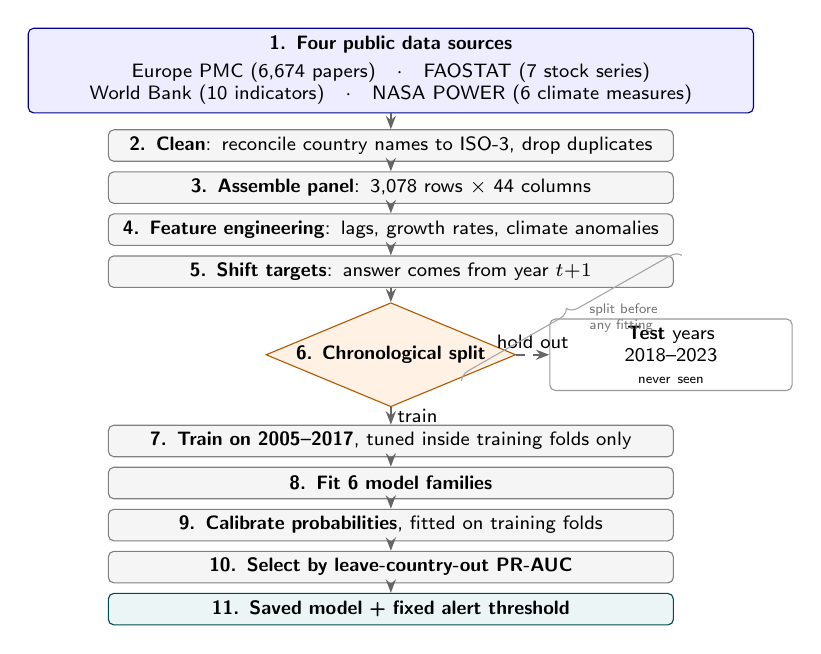
\begin{tikzpicture}[
  st/.style={rectangle,rounded corners=2pt,draw=black!50,fill=black!4,
             align=center,minimum height=0.40cm,text width=7.0cm,
             font=\scriptsize\sffamily,inner sep=2.5pt},
  srcbox/.style={rectangle,rounded corners=2pt,draw=blue!55!black,fill=blue!7,
             align=center,minimum height=0.80cm,text width=9.0cm,
             font=\scriptsize\sffamily,inner sep=3pt},
  dec/.style={diamond,draw=orange!70!black,fill=orange!10,aspect=2.4,
              align=center,font=\scriptsize\sffamily,inner sep=1pt},
  final/.style={rectangle,rounded corners=2pt,draw=teal!60!black,fill=teal!8,
             align=center,minimum height=0.40cm,text width=7.0cm,
             font=\scriptsize\sffamily,inner sep=2.5pt},
  testb/.style={rectangle,rounded corners=2pt,draw=black!40,fill=white,
             align=center,minimum height=0.52cm,text width=2.9cm,
             font=\scriptsize\sffamily,inner sep=2.5pt},
  fl/.style={-{Stealth[length=1.7mm]},thick,draw=black!60},
  step/.style={font=\scriptsize\sffamily\bfseries,text=black!45,anchor=east},
]

  \node[srcbox] (src) at (0,0)
    {\textbf{1. Four public data sources}\\[2pt]
     Europe PMC (6{,}674 papers)\quad$\cdot$\quad FAOSTAT (7 stock series)\\
     World Bank (10 indicators)\quad$\cdot$\quad NASA POWER (6 climate measures)};

  \node[st,below=0.20cm of src] (clean) {\textbf{2. Clean}: reconcile country names to ISO-3, drop duplicates};
  \node[st,below=0.12cm of clean] (panel) {\textbf{3. Assemble panel}: 3{,}078 rows $\times$ 44 columns};
  \node[st,below=0.12cm of panel] (feat) {\textbf{4. Feature engineering}: lags, growth rates, climate anomalies};
  \node[st,below=0.12cm of feat] (shift) {\textbf{5. Shift targets}: answer comes from year $t{+}1$};
  \node[dec,below=0.18cm of shift] (split) {\textbf{6. Chronological split}};

  % training branch (down)
  \node[st,below=0.22cm of split] (train) {\textbf{7. Train on 2005--2017}, tuned inside training folds only};
  \node[st,below=0.12cm of train] (fit) {\textbf{8. Fit 6 model families}};
  \node[st,below=0.12cm of fit] (cal) {\textbf{9. Calibrate probabilities}, fitted on training folds};
  \node[st,below=0.12cm of cal] (sel) {\textbf{10. Select by leave-country-out PR-AUC}};
  \node[final,below=0.12cm of sel] (saved) {\textbf{11. Saved model + fixed alert threshold}};

  % test branch (right)
  \node[testb,right=0.42cm of split] (test) {\textbf{Test} years\\2018--2023\\\tiny never seen};

  \draw[fl] (src) -- (clean);
  \draw[fl] (clean) -- (panel);
  \draw[fl] (panel) -- (feat);
  \draw[fl] (feat) -- (shift);
  \draw[fl] (shift) -- (split);
  \draw[fl] (split) -- node[font=\scriptsize\sffamily,right=1pt,inner sep=1pt] {train} (train);
  \draw[fl] (train) -- (fit);
  \draw[fl] (fit) -- (cal);
  \draw[fl] (cal) -- (sel);
  \draw[fl] (sel) -- (saved);
  \draw[fl,dashed] (split.east) -- node[font=\scriptsize\sffamily,above,inner sep=2pt] {hold out} (test.west);

  % brace showing where leakage protection sits
  \draw[decorate,decoration={brace,amplitude=4pt,mirror},black!35]
       ([xshift=0.10cm]shift.north east) -- ([xshift=0.10cm]split.south east)
       node[midway,right=3pt,font=\tiny\sffamily,text=black!55,align=left]
       {split before\\any fitting};
\end{tikzpicture}
\caption{Training pipeline. The chronological split sits before any model sees the
data, so the 2018--2023 years never influence training. Tuning and calibration both
happen strictly inside the training years.}
\label{fig:trainflow}
\end{figure}


% =====================================================================
\section{How The Maths Works}
\label{sec:maths}

Four ideas carry most of the analysis.

\paragraph{Precision and recall.} The model flags some rows as risky. \emph{Precision}
asks what share of the flagged rows were real, and \emph{recall} asks what share of the real
events we flagged. They pull against each other, since flagging more rows raises recall and
lowers precision. \emph{F1} combines the two. For an alert system this trade-off is the
whole design decision: a missed outbreak costs lives, and crying wolf costs attention,
because owners stop reading.

\paragraph{Why PR-AUC instead of accuracy.} Sort every row by predicted risk, walking from
most to least risky, and at each step compute precision and recall. The area under that
curve is PR-AUC, which answers how quickly picking the riskiest rows surfaces real events. A
method with no skill scores the prevalence, 0.056 here. The 2,906 easy negative rows cannot
inflate it, which is why it suits rare events. ROC-AUC has the opposite weakness: the large
negative class makes a mediocre model look strong. We report it so our numbers can be
compared with other papers.

\paragraph{Calibration.} A ranking can sort countries, but a message quoting a ``30\%
chance'' needs that number to be true. We group predictions into buckets and compare each
bucket's average prediction with how often the event happened. The averaged gap is
the expected calibration error, or 0.025, which is 0.025 here. The correction is fitted on
training data only, and it never reorders rows, only the numbers on the axis.

\paragraph{SHAP.} SHAP comes from cooperative game theory. If each feature were a player
contributing to a prediction, what is each player's fair share of the credit? Fair here
means averaging the contribution over every possible order in which features could be
added. One property makes it far more useful than simpler measures:

\begin{quote}
\small The contributions add up exactly to the gap between the model's average prediction
and this particular prediction.
\end{quote}

That property is called local accuracy. It lets us say that a prediction is 54\% rather
than the 5.6\% average, and give the exact breakdown of why, with nothing left over.


\begin{figure}[htbp]
\centering
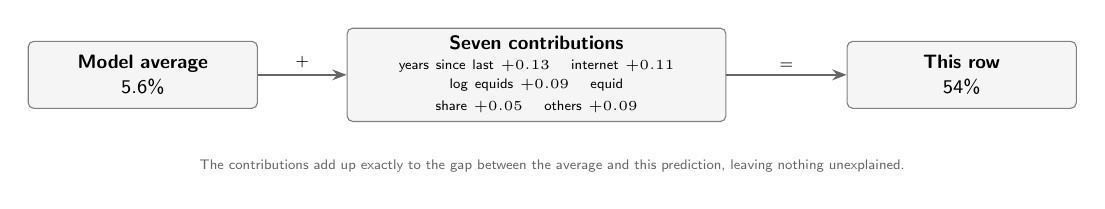
\begin{tikzpicture}[
  bx/.style={rectangle,rounded corners=2pt,draw=black!50,fill=black!4,
             align=center,font=\scriptsize\sffamily,inner sep=3pt},
  fl/.style={-{Stealth[length=1.8mm]},thick,draw=black!60},
]
  \node[bx,text width=2.7cm,minimum height=0.85cm] (a) at (0,0)
       {\textbf{Model average}\\[1pt]5.6\%};
  \node[bx,text width=4.6cm,minimum height=0.85cm] (b) at (5.0,0)
       {\textbf{Seven contributions}\\[1pt]\tiny years since last $+0.13$
        \quad internet $+0.11$\\[-1pt]\tiny log equids $+0.09$ \quad
        equid share $+0.05$ \quad others $+0.09$};
  \node[bx,text width=2.7cm,minimum height=0.85cm] (c) at (10.4,0)
       {\textbf{This row}\\[1pt]54\%};

  \draw[fl] (a) -- node[font=\tiny\sffamily,above,inner sep=2pt]{$+$} (b);
  \draw[fl] (b) -- node[font=\tiny\sffamily,above,inner sep=2pt]{$=$} (c);

  \node[font=\tiny\sffamily,text=black!60,anchor=north,text width=12.4cm,align=center]
       at (5.2,-0.95)
       {The contributions add up exactly to the gap between the average and this
        prediction, leaving nothing unexplained.};
\end{tikzpicture}
\caption{SHAP attributes one prediction to its inputs. Because the contributions must
sum exactly to the gap, the explanation is arithmetic rather than a plausible story.}
\label{fig:shap}
\end{figure}


SHAP distributes credit \emph{inside} the model. When two features carry the same
information the split between them is arbitrary, and a large value is not evidence of
cause.

% =====================================================================
\section{Results}
\label{sec:results}
% =====================================================================

\begin{table}[htbp]
\centering
\caption{Main results. Every column except Precision and Recall is a 0 to 1 score where
higher is better. The first four columns come from the time split, where the model is tested
on later years. The fifth repeats the main score under the harder country split, where the
model is tested on unseen countries. Precision and Recall describe what happens at the
alert threshold on the time split.}
\small
\resizebox{\textwidth}{!}{%
\begin{tabular}{@{}lcccccc@{}}
\toprule
\textbf{Model} & \textbf{PR-AUC} & \textbf{95\% interval} & \textbf{ROC-AUC} &
\textbf{PR-AUC} & \textbf{Precision} & \textbf{Recall} \\
 & \textbf{(time split)} & \textbf{on PR-AUC} & \textbf{(time split)} &
\textbf{(country split)} & \textbf{(time split)} & \textbf{(time split)} \\
\midrule
Logistic regression & 0.446 & [0.34, 0.57] & 0.863 & 0.336 & 0.30 & 0.65 \\
Decision tree & 0.424 & [0.32, 0.53] & 0.860 & 0.240 & 0.44 & 0.49 \\
Random forest & 0.518 & [0.40, 0.63] & 0.865 & 0.318 & 0.52 & 0.49 \\
Extra trees & 0.516 & [0.41, 0.62] & 0.860 & 0.284 & 0.46 & 0.51 \\
XGBoost & 0.432 & [0.32, 0.55] & 0.842 & 0.292 & 0.52 & 0.43 \\
LightGBM & 0.452 & [0.34, 0.57] & 0.840 & 0.311 & 0.58 & 0.38 \\
\bottomrule
\end{tabular}}
\end{table}

The two PR-AUC columns measure the same thing on different tests. Time split trains on 2005
to 2017 and tests on 2018 to 2023. Country split trains without some countries and tests on
those, which is harder and closer to real use. Neither is a precision score.

PR-AUC sits at 0.056 for a model with no skill. On the time split the best model reaches
0.518; on the country split, which is closer to real use, the logistic regression leads at
0.336. The uncertainty column is wide: with 74 positives in the test years a score can
move a long way within that range, so neighbouring models should not be separated with
confidence.

The ensembles lead on the time split, but on the country split the logistic regression is
ahead, and the single tree comes last on both. With only fourteen inputs the relationships are
close enough to additive that a regularised linear model transfers best.



\begin{multicols}{3}
\begin{thebibliography}{99}
\tiny
\setlength{\itemsep}{0.15em}
\setlength{\parskip}{0pt}
\bibitem{khan2013} Khan I, Wieler LH, Melzer F, et al. Glanders in animals: a review on epidemiology, clinical presentation, diagnosis and countermeasures. \emph{Transboundary and Emerging Diseases}. 2013. doi:10.1111/j.1865-1682.2012.01342.x
\bibitem{kanani2026} Kanani Y, Oryan A, Derakhshandeh A. Glanders: past, present and future of a neglected zoonosis as a threat in veterinary and human health. \emph{Veterinary Medicine and Science}. 2026. doi:10.1002/vms3.70950
\bibitem{purnama2026} Purnama MTE, Firdausy LW, Fikri F, et al. Seroprevalence and associated epidemiological drivers of glanders in horses: a systematic review and meta-analysis. \emph{Research in Veterinary Science}. 2026;106416. doi:10.1016/j.rvsc.2026.106416
\bibitem{mota2022} Mota RA, Pinheiro J\'unior JW. Current status of glanders in Brazil: recent advances and challenges. \emph{Brazilian Journal of Microbiology}. 2022. doi:10.1007/s42770-022-00814-1
\bibitem{singha2026} Singha H, Shanmugasundaram K, Jhandai P, et al. Surveillance of equine glanders in India (2019--2023): prevalence estimate, risk analysis and future strategy. \emph{Microbial Pathogenesis}. 2026;217:108597. doi:10.1016/j.micpath.2026.108597
\bibitem{singha2020} Singha H, Shanmugasundaram K, Tripathi BN, et al. Serological surveillance and clinical investigation of glanders among indigenous equines in India from 2015 to 2018. \emph{Transboundary and Emerging Diseases}. 2020. doi:10.1111/tbed.13475
\bibitem{malik2012} Malik P, Singha H, Khurana SK, et al. Emergence and re-emergence of glanders in India: a description of outbreaks from 2006 to 2011. \emph{Veterinaria Italiana}. 2012. PMID:22718333
\bibitem{fonseca2019} Fonseca-Rodr\'iguez O, Pinheiro J\'unior JW, Mota RA. Spatiotemporal analysis of glanders in Brazil. \emph{Journal of Equine Veterinary Science}. 2019. doi:10.1016/j.jevs.2019.03.216
\bibitem{hollings2017} Hollings T, Robinson A, van Andel M, et al. Species distribution models: a comparison of statistical approaches for livestock and disease epidemics. \emph{PLOS ONE}. 2017;12(8):e0183626. doi:10.1371/journal.pone.0183626
\bibitem{alshatti2026} Alshatti M, Al-Hemoud A, Othman A, et al. A risk prediction model for highly pathogenic avian influenza outbreaks in Kuwait. \emph{Frontiers in Veterinary Science}. 2026. doi:10.3389/fvets.2026.1843962
\bibitem{kane2014} Kane MJ, Price N, Scotch M, Rabinowitz P. Comparison of ARIMA and Random Forest time series models for prediction of avian influenza H5N1 outbreaks. \emph{BMC Bioinformatics}. 2014;15:276. doi:10.1186/1471-2105-15-276
\bibitem{walsh2019} Walsh DP, Ma TF, Ip HS, Zhu J. Artificial intelligence and avian influenza: using machine learning to enhance active surveillance for avian influenza viruses. \emph{Transboundary and Emerging Diseases}. 2019. doi:10.1111/tbed.13318
\bibitem{yoo2022} Yoo DS, Song YH, Choi DW, et al. Machine learning-driven dynamic risk prediction for highly pathogenic avian influenza at poultry farms in the Republic of Korea. \emph{Transboundary and Emerging Diseases}. 2021. doi:10.1111/tbed.14419
\bibitem{moawad2019} Moawad AA, Silge A, Bocklitz T, Fischer K, R\"osch P, Roesler U, Elschner MC, Popp J, Neubauer H. A machine learning-based Raman spectroscopic assay for the identification of \emph{Burkholderia mallei} and related species. \emph{Molecules}. 2019;24(24):4516. doi:10.3390/molecules24244516
\bibitem{stoeckel2015} St\"ockel S, Meisel S, Elschner M, Melzer F, R\"osch P, Popp J. Raman spectroscopic detection and identification of \emph{Burkholderia mallei} and \emph{Burkholderia pseudomallei}. \emph{Analytical and Bioanalytical Chemistry}. 2015;407(3):833--843. doi:10.1007/s00216-014-7906-5
\bibitem{collier2012} Collier N. Uncovering text mining: a survey of current work on web-based epidemic intelligence. \emph{Global Public Health}. 2012. doi:10.1080/17441692.2012.699975
\bibitem{lejeune2015} Lejeune G, Brixtel R, Doucet A, et al. Multilingual event extraction for epidemic detection. \emph{Artificial Intelligence in Medicine}. 2015. doi:10.1016/j.artmed.2015.06.005
\bibitem{chen2016} Chen T, Guestrin C. XGBoost: a scalable tree boosting system. In: \emph{Proceedings of the 22nd ACM SIGKDD International Conference on Knowledge Discovery and Data Mining}. 2016:785--794. doi:10.1145/2939672.2939785
\bibitem{ke2017} Ke G, Meng Q, Finley T, et al. LightGBM: a highly efficient gradient boosting decision tree. In: \emph{Advances in Neural Information Processing Systems 30 (NIPS)}. 2017:3146--3154.
\bibitem{breiman2001} Breiman L. Random forests. \emph{Machine Learning}. 2001. doi:10.1023/A:1010933404324
\bibitem{lundberg2017} Lundberg SM, Lee SI. A unified approach to interpreting model predictions. In: \emph{Advances in Neural Information Processing Systems 30 (NIPS)}. 2017:4765--4774. arXiv:1705.07874
\bibitem{saito2015} Saito T, Rehmsmeier M. The precision-recall plot is more informative than the ROC plot when evaluating binary classifiers on imbalanced datasets. \emph{PLOS ONE}. 2015;10(3):e0118432. doi:10.1371/journal.pone.0118432
\bibitem{davis2006} Davis J, Goadrich M. The relationship between precision-recall and ROC curves. In: \emph{Proceedings of the 23rd International Conference on Machine Learning}. 2006:233--240. doi:10.1145/1143844.1143874
\bibitem{roberts2017} Roberts DR, Bahn V, Ciuti S, et al. Cross-validation strategies for data with temporal, spatial, hierarchical, or phylogenetic structure. \emph{Ecography}. 2017. doi:10.1111/ecog.02881
\bibitem{niculescu2005} Niculescu-Mizil A, Caruana R. Predicting good probabilities with supervised learning. In: \emph{Proceedings of the 22nd International Conference on Machine Learning}. 2005:625--632. doi:10.1145/1102351.1102430
\bibitem{huang2020} Huang Y, Li W, Macheret F, et al. A tutorial on calibration measurements and calibration models for clinical prediction models. \emph{Journal of the American Medical Informatics Association}. 2020;27(4):621--633. doi:10.1093/jamia/ocz228
\bibitem{lewis2020} Lewis P, Perez E, Piktus A, et al. Retrieval-augmented generation for knowledge-intensive NLP tasks. In: \emph{Advances in Neural Information Processing Systems 33 (NeurIPS)}. 2020:9459--9474. arXiv:2005.11401
\bibitem{reimers2019} Reimers N, Gurevych I. Sentence-BERT: sentence embeddings using Siamese BERT-networks. In: \emph{Proceedings of the 2019 Conference on Empirical Methods in Natural Language Processing (EMNLP-IJCNLP)}. 2019:3982--3992. doi:10.18653/v1/D19-1410
\bibitem{malkov2020} Malkov YA, Yashunin DA. Efficient and robust approximate nearest neighbor search using hierarchical navigable small world graphs. \emph{IEEE Transactions on Pattern Analysis and Machine Intelligence}. 2020;42(4):824--836. doi:10.1109/TPAMI.2018.2889473
\bibitem{robertson2009} Robertson S, Zaragoza H. The probabilistic relevance framework: BM25 and beyond. \emph{Foundations and Trends in Information Retrieval}. 2009;3(4):333--389. doi:10.1561/1500000019
\bibitem{cormack2009} Cormack GV, Clarke CLA, Buettcher S. Reciprocal rank fusion outperforms Condorcet and individual rank learning methods. In: \emph{Proceedings of the 32nd International ACM SIGIR Conference}. 2009:758--759. doi:10.1145/1571941.1572114
\bibitem{pedregosa2011} Pedregosa F, Varoquaux G, Gramfort A, et al. Scikit-learn: machine learning in Python. \emph{Journal of Machine Learning Research}. 2011;12:2825--2830.
\bibitem{wahis} WOAH. World Animal Health Information System (WAHIS). \url{https://wahis.woah.org}
\bibitem{dahd2025} Department of Animal Husbandry and Dairying, Government of India. \emph{National Action Plan for Control and Eradication of Glanders in India} (Revised 2025). New Delhi: DAHD; 2025.
\bibitem{faostat} FAO. FAOSTAT: crops and livestock products. \url{https://www.fao.org/faostat}
\bibitem{power} NASA Langley Research Center. POWER agroclimatology API. \url{https://power.larc.nasa.gov}
\bibitem{wdi} World Bank. World Development Indicators. \url{https://databank.worldbank.org}
\bibitem{europepmc} Europe PMC literature search API. \url{https://europepmc.org}
\bibitem{nadres} ICAR-National Institute of Veterinary Epidemiology and Disease Informatics. National Animal Disease Referral Expert System (NADRES v2): livestock disease forecasting. \url{https://nivedi.res.in/Nadres_v2/}
\end{thebibliography}
\end{multicols}

\end{document}
